\documentclass[10pt]{article}

%Math
\usepackage{amsmath}
\usepackage{amsfonts}
\usepackage{amssymb}
\usepackage{amsthm}
\usepackage{ulem}
\usepackage{stmaryrd} %f\UTF{00FC}r Blitz!

%PageStyle
\usepackage[ngerman]{babel} % deutsche Silbentrennung
\usepackage[utf8]{inputenc} 
\usepackage{fancyhdr, graphicx}
\usepackage[scaled=0.92]{helvet}
\usepackage{enumitem}
\usepackage{parskip}
\usepackage[a4paper,top=2cm]{geometry}
\setlength{\textwidth}{17cm}
\setlength{\oddsidemargin}{-0.5cm}

% Shortcommands
\newcommand{\Bold}[1]{\textbf{#1}} %Boldface
\newcommand{\Kursiv}[1]{\textit{#1}} %Italic
\newcommand{\T}[1]{\text{#1}} %Textmode
\newcommand{\Nicht}[1]{\T{\sout{$ #1 $}}} %Streicht Shit durch

%Arrows
\newcommand{\lra}{\leftrightarrow} 
\newcommand{\ra}{\rightarrow}
\newcommand{\la}{\leftarrow}
\newcommand{\lral}{\longleftrightarrow}
\newcommand{\ral}{\longrightarrow}
\newcommand{\lal}{\longleftarrow}
\newcommand{\Lra}{\Leftrightarrow}
\newcommand{\Ra}{\Rightarrow}
\newcommand{\La}{\Leftarrow}
\newcommand{\Lral}{\Longleftrightarrow}
\newcommand{\Ral}{\Longrightarrow}
\newcommand{\Lal}{\Longleftarrow}

% Code listenings
\usepackage{color}
\usepackage{xcolor}
\usepackage{listings}
\usepackage{caption}
\DeclareCaptionFont{white}{\color{black}}
\DeclareCaptionFormat{listing}{\colorbox{white}{\parbox{\textwidth}{#1#2#3}}}
\captionsetup[lstlisting]{format=listing,labelfont=white,textfont=white,font=bf}


\lstdefinestyle{sqlNoTitle}{
   language=SQL,
   basicstyle=\footnotesize\ttfamily, % Standardschrift
   backgroundcolor=\color[RGB]{230,230,230}, % Hintergrundfarbe
   numbers=left,               % Ort der Zeilennummern
   numberstyle=\tiny,          % Stil der Zeilennummern
   stepnumber=1,               % Abstand zwischen den Zeilennummern
   numbersep=5pt,              % Abstand der Nummern zum Text
   tabsize=2,                  % Groesse von Tabs
   extendedchars=true,         %
   breaklines=true,            % Zeilen werden Umgebrochen
   frame=trbl,                 % Rahmen
   stringstyle=\color[RGB]{42,0,255} \ttfamily, % Farbe der String
   keywordstyle=\color[RGB]{127,0,85} \ttfamily, % Farbe der Keywords
   commentstyle=\color[RGB]{63,127,95} \ttfamily, % Farbe des Kommentars
   showspaces=false,           % Leerzeichen anzeigen ?
   showtabs=false,             % Tabs anzeigen ?
   xleftmargin=17pt,
   framexleftmargin=17pt,
   framexrightmargin=5pt,
   framexbottommargin=5pt,
   framextopmargin=5pt,
   showstringspaces=false,     % Leerzeichen in Strings anzeigen ?
}


\lstdefinestyle{sql}{
   style=sqlNoTitle,
   title=SQL-Query
}

\lstdefinestyle{queryexecutionplan}{
  basicstyle=\footnotesize\ttfamily, % Standardschrift
  backgroundcolor=\color[RGB]{240,255,240}, % Hintergrundfarbe
  frame=trbl,                 % Rahmen
  title=Ausführungsplan
}

\lstdefinestyle{queryexecutionplanSmall}{
  style=queryexecutionplan,
  basicstyle=\scriptsize\ttfamily, % Standardschrift
}

%Config
\renewcommand{\headrulewidth}{0pt}
\setlength{\headheight}{15.2pt}

%Metadata
\fancyfoot[C]{}
\title{
	\vspace{4cm}
	\huge{Datenbank-Architektur für Fortgeschrittene}\\
	\vspace{0.2cm}
	\Large{Ausarbeitung 1: Anfrageverarbeitung}\\
}
\author{Thomas Baumann / Egemen Kaba}
\date{03. Mai 2013}

% hier beginnt das Dokument
\begin{document}

% Titelbild
\maketitle
\thispagestyle{fancy}

\newpage

% Inhaltsverzeichnis
\pagenumbering{Roman}
\tableofcontents	  	


\newpage
\setcounter{page}{1}
\pagenumbering{arabic}

% Inhalt Start

\section{Einleitung}
Die Ausarbeitung haben wir mit folgender Datenbankverbindung ausgeführt.

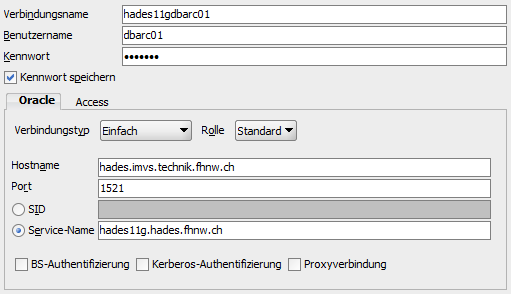
\includegraphics{login_daten.png}

\section{Vorbereitung}
\subsection{Einrichten Datenbasis}
Die Datenbank haben wir mit folgenden Querys eingerichtet.
\begin{lstlisting}[style=sql]
CREATE TABLE regions
AS SELECT *
  FROM dbarc00.regions;
  
CREATE TABLE nations
AS SELECT *
  FROM dbarc00.nations;

CREATE TABLE parts
AS SELECT *
  FROM dbarc00.parts;
  
CREATE TABLE customers
AS SELECT *
  FROM dbarc00.customers;

CREATE TABLE suppliers
AS SELECT *
  FROM dbarc00.suppliers;

CREATE TABLE orders
AS SELECT *
  FROM dbarc00.orders;

CREATE TABLE partsupps
AS SELECT *
  FROM dbarc00.partsupps;

CREATE TABLE lineitems
AS SELECT *
  FROM dbarc00.lineitems;
\end{lstlisting}
\subsection{Tabellenstatistik}
\begin{lstlisting}[style=sql]
SELECT segment_name, bytes, blocks, extents
FROM user_segments;

SELECT table_name, num_rows
FROM user_tab_statistics;
\end{lstlisting}
Folgende Tabellenstatistik haben wir mit den oben genannten Querys erhoben.
\begin{tabular}{l||r|r|r|r}
  Tabelle & Anzahl Zeilen & Grösse in Bytes & Anzahl Blöcke & Anzahl Extents \\ \hline
  \hline
  CUSTOMERS & 150'000 & 29'360'128 & 3'584 & 43 \\ \hline
  LINEITEMS & 6'001'215 & 897'581'056 & 109'568 & 178 \\ \hline
  NATIONS & 25 & 65'536 & 8 & 1 \\ \hline
  ORDERS & 1'500'000 & 201'326'592 & 24'576 & 95 \\ \hline
  PARTS & 200'000 & 32'505'856 & 3'968 & 46 \\ \hline
  PARTSUPPS & 800'000 & 142'606'336 & 17'408 & 88 \\ \hline
  REGIONS & 5 & 65'536 & 8 & 1 \\ \hline
  SUPPLIERS & 10'000 & 2'097'152 & 256 & 17 \\
\end{tabular}	
Je nachdem, wo man die Werte ausliest, erhält man andere Werte für die Grösse und 
Anzahl Blöcke.
\section{Ausführungsplan}
\begin{lstlisting}[style=sql]
EXPLAIN PLAN FOR
SELECT *
FROM parts;

SELECT plan_table_output
FROM TABLE(DBMS_XPLAN.DISPLAY('plan_table',null,'serial'));
\end{lstlisting}
\begin{lstlisting}[style=queryexecutionplan]
---------------------------------------------------------------------------
| Id  | Operation         | Name  | Rows  | Bytes | Cost (%CPU)| Time     |
---------------------------------------------------------------------------
|   0 | SELECT STATEMENT  |       |   190K|    26M|  1051   (1)| 00:00:13 |
|   1 |  TABLE ACCESS FULL| PARTS |   190K|    26M|  1051   (1)| 00:00:13 |
---------------------------------------------------------------------------
\end{lstlisting}
Die Tabelle zeigt die einzelnen Schritte des Ausführungsplanes, welche der 
Optimizer erstellt hat, mit den jeweilig zurückgegebenen Anzahl Zeilen, deren 
Grösse, die Kosten und Zeit für die Teilschritte. Man kann sich den 
Ausführungsplan als Baum vorstellen. Die Einrückungen stellen die Knotentiefe 
dar. Die Kosten für einen Elternknoten werden aus der Summe der Kosten der 
Kindknoten plus die eigenen Kosten berechnet.

Für die nächsten Aufgaben verwenden wir das obenstehende Statement. Wir 
haben jeweils das Query ausgetauscht um den Ausführungsplan zu erhalten.

\section{Versuche ohne Index}
\subsection{Projektion}
\begin{lstlisting}[style=sql]
SELECT *
FROM orders;
\end{lstlisting}
\begin{lstlisting}[style=queryexecutionplan]
----------------------------------------------------------------------------
| Id  | Operation         | Name   | Rows  | Bytes | Cost (%CPU)| Time     |
----------------------------------------------------------------------------
|   0 | SELECT STATEMENT  |        |  1579K|   209M|  6612   (1)| 00:01:20 |
|   1 |  TABLE ACCESS FULL| ORDERS |  1579K|   209M|  6612   (1)| 00:01:20 |
---------------------------------------------------------------------------- 
\end{lstlisting}   
\textbf{Reflexion} \newline
Da alle Zeilen und Spalten der Tabelle ausgelesen werden müssen, wird hier ein
Full Table Scan durchgeführt. Da alle Spalten verwendet werden, muss keine Projektion 
vorgenommen werden.

\begin{lstlisting}[style=sql]
SELECT o_clerk
FROM orders;
\end{lstlisting}
\begin{lstlisting}[style=queryexecutionplan]
----------------------------------------------------------------------------
| Id  | Operation         | Name   | Rows  | Bytes | Cost (%CPU)| Time     |
----------------------------------------------------------------------------
|   0 | SELECT STATEMENT  |        |  1579K|    25M|  6608   (1)| 00:01:20 |
|   1 |  TABLE ACCESS FULL| ORDERS |  1579K|    25M|  6608   (1)| 00:01:20 |
---------------------------------------------------------------------------- 
\end{lstlisting}   
\textbf{Reflexion} \newline
Es werden wiederum alle Zeile, jedoch nicht alle Spalten ausgelesen.
Exakt läuft es so ab, dass zuerst die ganze Tabelle gelesen wird und danach die nicht
benötigten Spalten herausgefiltert werden.
Das verringert die Anzahl Daten, die gespeichert werden müssen, drastisch von 209MB auf 25MB.

\begin{lstlisting}[style=sql]
SELECT DISTINCT o_clerk
FROM orders;
\end{lstlisting}
\begin{lstlisting}[style=queryexecutionplan]
-------------------------------------------------------------------------------------
| Id  | Operation          | Name   | Rows  | Bytes |TempSpc| Cost (%CPU)| Time     |
-------------------------------------------------------------------------------------
|   0 | SELECT STATEMENT   |        |  1579K|    25M|       | 15333   (1)| 00:03:04 |
|   1 |  HASH UNIQUE       |        |  1579K|    25M|    36M| 15333   (1)| 00:03:04 |
|   2 |   TABLE ACCESS FULL| ORDERS |  1579K|    25M|       |  6608   (1)| 00:01:20 |
-------------------------------------------------------------------------------------
\end{lstlisting} 
\textbf{Reflexion} \newline
Wie beim vorherigen Befehl werden alle Zeilen einer bestimmten Spalte ausgelesen,
was wiederum einen Zugriff auf die gesamte Tabelle nötig macht.
Zusätzlich zu diesem Aufwand müssen alle doppelten Einträge herausgefiltert werden,
was die massiv angestiegenen CPU-Kosten bei Operation 1 erklärt.
Für die Speicherung von Zwischenresultaten wird dabei temporärer Speicher beansprucht.

\subsection{Selektion}
\begin{lstlisting}[style=sql]
SELECT *
FROM orders
WHERE o_orderkey = 44444;
\end{lstlisting}
\begin{lstlisting}[style=queryexecutionplan]
----------------------------------------------------------------------------
| Id  | Operation         | Name   | Rows  | Bytes | Cost (%CPU)| Time     |
----------------------------------------------------------------------------
|   0 | SELECT STATEMENT  |        |   267 | 37113 |  6603   (1)| 00:01:20 |
|*  1 |  TABLE ACCESS FULL| ORDERS |   267 | 37113 |  6603   (1)| 00:01:20 |
----------------------------------------------------------------------------

Predicate Information (identified by operation id):
---------------------------------------------------
   1 - filter("O_ORDERKEY"=44444)
\end{lstlisting}
\textbf{Reflexion} \newline
Es soll nur ein Tupel ausgewählt werden (Spalte ist Primary Key), da jedoch 
kein index besteht, ist nicht bekannt, welches der Eintrag ist und zusätzlich 
kann nach dem ersten Fund nicht abgebrochen werden. Deshalb muss wieder ein 
Full Table Scan durchgeführt werden. Durch die Bedingung wird viel weniger 
Hauptspeicher benötigt.

\begin{lstlisting}[style=sql]
SELECT *
FROM orders
WHERE o_orderkey = 44444 OR o_clerk = 'Clerk#000000286';
\end{lstlisting}
\begin{lstlisting}[style=queryexecutionplan]
----------------------------------------------------------------------------
| Id  | Operation         | Name   | Rows  | Bytes | Cost (%CPU)| Time     |
----------------------------------------------------------------------------
|   0 | SELECT STATEMENT  |        |   267 | 37113 |  6631   (1)| 00:01:20 |
|*  1 |  TABLE ACCESS FULL| ORDERS |   267 | 37113 |  6631   (1)| 00:01:20 |
----------------------------------------------------------------------------

Predicate Information (identified by operation id):
---------------------------------------------------
   1 - filter("O_ORDERKEY"=44444 OR "O_CLERK"='Clerk#000000286')
\end{lstlisting}
\textbf{Reflexion} \newline
Im Vergleich zum vorherigen Query sind nur die Kosten minimal gestiegen, dies 
ist auf die zweite Bedingung zurück zu führen.

\begin{lstlisting}[style=sql]
SELECT *
FROM orders
WHERE o_orderkey = 44444 AND o_clerk = 'Clerk#000000286';
\end{lstlisting}
\begin{lstlisting}[style=queryexecutionplan]
----------------------------------------------------------------------------
| Id  | Operation         | Name   | Rows  | Bytes | Cost (%CPU)| Time     |
----------------------------------------------------------------------------
|   0 | SELECT STATEMENT  |        |   158 | 21962 |  6612   (1)| 00:01:20 |
|*  1 |  TABLE ACCESS FULL| ORDERS |   158 | 21962 |  6612   (1)| 00:01:20 |
----------------------------------------------------------------------------

Predicate Information (identified by operation id):
---------------------------------------------------
   1 - filter("O_ORDERKEY"=44444 AND "O_CLERK"='Clerk#000000286')
\end{lstlisting}
\textbf{Reflexion} \newline
Durch die AND-verknüpfung muss die zweite Bedingung nur überprüft werden, wenn 
die Erste erfüllt ist. So sind alle Werte, ausser der Zeit gesunken.

\begin{lstlisting}[style=sql]
SELECT *
FROM orders
WHERE o_orderkey*2 = 44444 AND o_clerk = 'Clerk#000000286';
\end{lstlisting}
\begin{lstlisting}[style=queryexecutionplan]
----------------------------------------------------------------------------
| Id  | Operation         | Name   | Rows  | Bytes | Cost (%CPU)| Time     |
----------------------------------------------------------------------------
|   0 | SELECT STATEMENT  |        |   158 | 21962 |  6616   (1)| 00:01:20 |
|*  1 |  TABLE ACCESS FULL| ORDERS |   158 | 21962 |  6616   (1)| 00:01:20 |
----------------------------------------------------------------------------

Predicate Information (identified by operation id):
---------------------------------------------------
   1 - filter("O_ORDERKEY"*2=44444 AND "O_CLERK"='Clerk#000000286')
\end{lstlisting}
\textbf{Reflexion} \newline
Die Werte sind alle genau gleich, wie beim vorherigen Query, obwohl eigentlich 
eine zusätzliche Operation pro Zeile notwendig ist ($o\_orderkey*2$). Wir 
vermuten, dass dieses Query vor der Abfrage optimiert wird, besser gesagt, die
Berechnung wird vereinfacht, so muss nur eine Operation ausgeführt werden:
\begin{lstlisting}[style=sqlNoTitle]
o_orderkey = 22222 AND o_clerk = 'Clerk#000000286'
\end{lstlisting}

\begin{lstlisting}[style=sql]
SELECT *
FROM orders
WHERE o_orderkey BETWEEN 111111 AND 222222;
\end{lstlisting}
\begin{lstlisting}[style=queryexecutionplan]
----------------------------------------------------------------------------
| Id  | Operation         | Name   | Rows  | Bytes | Cost (%CPU)| Time     |
----------------------------------------------------------------------------
|   0 | SELECT STATEMENT  |        |   267 | 37113 |  6603   (1)| 00:01:20 |
|*  1 |  TABLE ACCESS FULL| ORDERS |   267 | 37113 |  6603   (1)| 00:01:20 |
----------------------------------------------------------------------------

Predicate Information (identified by operation id):
---------------------------------------------------
   1 - filter("O_ORDERKEY">=111111 AND "O_ORDERKEY"<=222222)
\end{lstlisting}
\textbf{Reflexion} \newline

Die Selektion 
\begin{lstlisting}[style=sqlNoTitle]
column BETWEEN x AND y 
\end{lstlisting}
wird durch folgendes 
\begin{lstlisting}[style=sqlNoTitle]
column >= x AND column <= y 
\end{lstlisting}
ersetzt. Im Vergleich zum Vorherigen, sind die Anzahl Zeilen und die 
Speicherbenutzung gestiegen, dies weil mehr Tupel selektiert werden. Hingegen 
sind die Kosten minimal gesunken, da die beiden Vergleiche auf der gleichen 
Spalte vorgenommen werden.

\begin{lstlisting}[style=sql]
SELECT *
FROM orders
WHERE o_orderkey BETWEEN 44444 AND 55555
AND o_clerk BETWEEN 'Clerk#000000130' AND 'Clerk#000000139';
\end{lstlisting}
\begin{lstlisting}[style=queryexecutionplan]
----------------------------------------------------------------------------
| Id  | Operation         | Name   | Rows  | Bytes | Cost (%CPU)| Time     |
----------------------------------------------------------------------------
|   0 | SELECT STATEMENT  |        |    10 |  1390 |  6613   (1)| 00:01:20 |
|*  1 |  TABLE ACCESS FULL| ORDERS |    10 |  1390 |  6613   (1)| 00:01:20 |
----------------------------------------------------------------------------

Predicate Information (identified by operation id):
---------------------------------------------------
   1 - filter("O_ORDERKEY">=44444 AND "O_ORDERKEY"<=55555 AND 
              "O_CLERK">='Clerk#000000130' AND "O_CLERK"<='Clerk#000000139')
\end{lstlisting}
\textbf{Reflexion} \newline
Auch hier wurden die BETWEEN-Statements mit grösser gleich und kleiner gleich 
ersetzt. Die Resultierende Anzahl Tupel und der benötigte Speicher sind nochmals 
gesunken. Wohin gegen die Kosten gestiegen sind, da bis zu vier Vergleiche 
notwendig sind.

\subsection{Join}
\begin{lstlisting}[style=sql]
SELECT *
FROM orders, customers
WHERE o_custkey = c_custkey
AND o_orderkey < 100;
\end{lstlisting}
\begin{lstlisting}[style=queryexecutionplan]
--------------------------------------------------------------------------------
| Id  | Operation          | Name      | Rows  | Bytes | Cost (%CPU)| Time     |
--------------------------------------------------------------------------------
|   0 | SELECT STATEMENT   |           |    25 |  6750 |  7555   (1)| 00:01:31 |
|*  1 |  HASH JOIN         |           |    25 |  6750 |  7555   (1)| 00:01:31 |
|*  2 |   TABLE ACCESS FULL| ORDERS    |    25 |  2775 |  6602   (1)| 00:01:20 |
|   3 |   TABLE ACCESS FULL| CUSTOMERS |   150K|    22M|   951   (1)| 00:00:12 |
--------------------------------------------------------------------------------

Predicate Information (identified by operation id):
---------------------------------------------------                                                                 
   1 - access("O_CUSTKEY"="C_CUSTKEY")
   2 - filter("O_ORDERKEY"<100)
\end{lstlisting}  
\textbf{Varianten}
\begin{lstlisting}[style=sql]
SELECT *
FROM customers, orders
WHERE o_orderkey < 100
AND c_custkey = o_custkey;
\end{lstlisting}
\begin{lstlisting}[style=queryexecutionplan]
--------------------------------------------------------------------------------
| Id  | Operation          | Name      | Rows  | Bytes | Cost (%CPU)| Time     |
--------------------------------------------------------------------------------
|   0 | SELECT STATEMENT   |           |    25 |  6750 |  7556   (1)| 00:01:31 |
|*  1 |  HASH JOIN         |           |    25 |  6750 |  7556   (1)| 00:01:31 |
|*  2 |   TABLE ACCESS FULL| ORDERS    |    25 |  2775 |  6604   (1)| 00:01:20 |
|   3 |   TABLE ACCESS FULL| CUSTOMERS |   150K|    22M|   951   (1)| 00:00:12 |
--------------------------------------------------------------------------------

Predicate Information (identified by operation id):
---------------------------------------------------
   1 - access("C_CUSTKEY"="O_CUSTKEY")
   2 - filter("O_ORDERKEY"<100)
\end{lstlisting}
\begin{lstlisting}[style=sql]
SELECT *
FROM customers, orders
WHERE c_custkey = o_custkey
AND o_orderkey < 100;
\end{lstlisting}
\begin{lstlisting}[style=queryexecutionplan]
--------------------------------------------------------------------------------
| Id  | Operation          | Name      | Rows  | Bytes | Cost (%CPU)| Time     |
--------------------------------------------------------------------------------
|   0 | SELECT STATEMENT   |           |    25 |  6750 |  7555   (1)| 00:01:31 |
|*  1 |  HASH JOIN         |           |    25 |  6750 |  7555   (1)| 00:01:31 |
|*  2 |   TABLE ACCESS FULL| ORDERS    |    25 |  2775 |  6602   (1)| 00:01:20 |
|   3 |   TABLE ACCESS FULL| CUSTOMERS |   150K|    22M|   951   (1)| 00:00:12 |
--------------------------------------------------------------------------------

Predicate Information (identified by operation id):
---------------------------------------------------
   1 - access("C_CUSTKEY"="O_CUSTKEY")
   2 - filter("O_ORDERKEY"<100)
\end{lstlisting}
\begin{lstlisting}[style=sql]
SELECT *
FROM customers, orders
WHERE o_custkey = c_custkey
AND o_orderkey < 100;
\end{lstlisting}
\begin{lstlisting}[style=queryexecutionplan]
--------------------------------------------------------------------------------
| Id  | Operation          | Name      | Rows  | Bytes | Cost (%CPU)| Time     |
--------------------------------------------------------------------------------
|   0 | SELECT STATEMENT   |           |    25 |  6750 |  7555   (1)| 00:01:31 |
|*  1 |  HASH JOIN         |           |    25 |  6750 |  7555   (1)| 00:01:31 |
|*  2 |   TABLE ACCESS FULL| ORDERS    |    25 |  2775 |  6602   (1)| 00:01:20 |
|   3 |   TABLE ACCESS FULL| CUSTOMERS |   150K|    22M|   951   (1)| 00:00:12 |
--------------------------------------------------------------------------------

Predicate Information (identified by operation id):
---------------------------------------------------
   1 - access("O_CUSTKEY"="C_CUSTKEY")
   2 - filter("O_ORDERKEY"<100)
\end{lstlisting}
\textbf{Reflexion} \newline
Der Optimizer wählt bei allen Varianten automatisch die Perfomanteste aus. Somit kann man 
sagen, dass die Rheinfolge in der WHERE Klausel keine Rolle spielt.

Es wird immer ein Full Table Scan auf die Tabelle orders mit der Selektion id=2 
vorgenommen, somit sind nur die benötigten Datensätze im Resultat. Das Resultat wird mit 
einem Hash Join mit der customers Tabelle vereinigt, welche mit einem Full Table Scan 
gelesen wurde. Da auf der Tabelle orders eine Selektion vorgenommen wird, wird diese 
Tabelle immer auf die Linke Seite des Joins genommen.

\section{Versuche mit Index}
Mit folgenden Befehlen wurden die Indizes erstellt.
\begin{lstlisting}[style=sql]
CREATE INDEX o_orderkey_ix ON orders(o_orderkey);
CREATE INDEX o_clerk_ix ON orders(o_clerk);
\end{lstlisting}

Mit folgendem Befehl wurden die Statistiken für die Indizes erhoben.
\begin{lstlisting}[style=sql]
SELECT segment_name, bytes
FROM user_segments;
\end{lstlisting}

\begin{tabular}{l||r|r|r}
  Index & Grösse in Bytes & Tabellen Grösse in Bytes & Anteil von \\ 
  & & &  Index an Tabelle \\ \hline
  \hline
  O\_ORDERKEY\_IX & 30'408'704 & 201'326'592 & 15.10\%  \\ \hline
  O\_CLERK\_IX & 48'234'496 & 201'326'592 & 23.96\% \\ 
\end{tabular}

\subsection{Projektion}
\begin{lstlisting}[style=sql]
SELECT DISTINCT o_clerk
FROM orders;
\end{lstlisting}
\begin{lstlisting}[style=queryexecutionplan]
------------------------------------------------------------------------------------
| Id  | Operation             | Name       | Rows  | Bytes | Cost (%CPU)| Time     |
------------------------------------------------------------------------------------
|   0 | SELECT STATEMENT      |            |  1000 | 16000 |  1622   (5)| 00:00:20 |
|   1 |  HASH UNIQUE          |            |  1000 | 16000 |  1622   (5)| 00:00:20 |
|   2 |   INDEX FAST FULL SCAN| O_CLERK_IX |  1500K|    22M|  1553   (1)| 00:00:19 |
------------------------------------------------------------------------------------
\end{lstlisting}
\textbf{Reflexion} \newline
Statt dem Full Table Scan wird jetzt ein Index Range Scan angewendet. Dadurch können 
die benötigten Tupel wesentlich schneller gefunden werden. Im Vergleich ohne Index 
werden nur minimal weniger Tupel ausgelesen, jedoch viel schneller. Hingegen der 
Hash Unique wird massiv schneller durchgearbeitet und liefert auch weniger Tupel zurück.
Bei beiden Projektionen beanspruchen keine Kosten.

\subsection{Selektion}
\begin{lstlisting}[style=sql]
SELECT *
FROM orders
WHERE o_orderkey = 44444;
\end{lstlisting}
\begin{lstlisting}[style=queryexecutionplan]
---------------------------------------------------------------------------------------------
| Id  | Operation                   | Name          | Rows  | Bytes | Cost (%CPU)| Time     |
---------------------------------------------------------------------------------------------
|   0 | SELECT STATEMENT            |               |     1 |   111 |     4   (0)| 00:00:01 |
|   1 |  TABLE ACCESS BY INDEX ROWID| ORDERS        |     1 |   111 |     4   (0)| 00:00:01 |
|*  2 |   INDEX RANGE SCAN          | O_ORDERKEY_IX |     1 |       |     3   (0)| 00:00:01 |
---------------------------------------------------------------------------------------------

Predicate Information (identified by operation id):
---------------------------------------------------
   2 - access("O_ORDERKEY"=44444)
\end{lstlisting}
\textbf{Reflexion} \newline
Hier wird selektiv mittels eines Index Range Scans gesucht. Es liefert die Position auf 
der Disk mittels der ROWID. Anhand dieser ROWID wird wiederum direkt auf die Tabelle 
zugegriffen.

\begin{lstlisting}[style=sql]
SELECT /*+ FULL(orders) */ *
FROM orders
WHERE o_orderkey = 44444;
\end{lstlisting}
\begin{lstlisting}[style=queryexecutionplan]
----------------------------------------------------------------------------
| Id  | Operation         | Name   | Rows  | Bytes | Cost (%CPU)| Time     |
----------------------------------------------------------------------------
|   0 | SELECT STATEMENT  |        |     1 |   111 |  6602   (1)| 00:01:20 |
|*  1 |  TABLE ACCESS FULL| ORDERS |     1 |   111 |  6602   (1)| 00:01:20 |
----------------------------------------------------------------------------

Predicate Information (identified by operation id):
---------------------------------------------------
   1 - filter("O_ORDERKEY"=44444)
\end{lstlisting}
\textbf{Reflexion} \newline
Der Hint erzwingt einen Full Table Scan, was zu einen massiven Anstieg des Ressourcenverbrauchs führt.\\
Der Index wird dabei nicht benutzt.

\begin{lstlisting}[style=sql]
SELECT *
FROM orders
WHERE o_orderkey = 44444 OR o_clerk = 'Clerk#000000286';
\end{lstlisting}
\begin{lstlisting}[style=queryexecutionplanSmall]
--------------------------------------------------------------------------------------------------
| Id  | Operation                        | Name          | Rows  | Bytes | Cost (%CPU)| Time     |
--------------------------------------------------------------------------------------------------
|   0 | SELECT STATEMENT                 |               |  1501 |   162K|   336   (0)| 00:00:05 |
|   1 |  TABLE ACCESS BY INDEX ROWID     | ORDERS        |  1501 |   162K|   336   (0)| 00:00:05 |
|   2 |   BITMAP CONVERSION TO ROWIDS    |               |       |       |            |          |
|   3 |    BITMAP OR                     |               |       |       |            |          |
|   4 |     BITMAP CONVERSION FROM ROWIDS|               |       |       |            |          |
|*  5 |      INDEX RANGE SCAN            | O_CLERK_IX    |       |       |     8   (0)| 00:00:01 |
|   6 |     BITMAP CONVERSION FROM ROWIDS|               |       |       |            |          |
|*  7 |      INDEX RANGE SCAN            | O_ORDERKEY_IX |       |       |     3   (0)| 00:00:01 |
--------------------------------------------------------------------------------------------------

Predicate Information (identified by operation id):
---------------------------------------------------
   5 - access("O_CLERK"='Clerk#000000286')
   7 - access("O_ORDERKEY"=44444)
\end{lstlisting}
\textbf{Reflexion} \newline
Durch den Zugriff auf Indizes wird auch hier direkt auf die benötigten Tupel zugegriffen.
Statt einer werden zwei Indizes verwendet, da die OR-Verknüpfung den Zugriff auf zwei indexierte Spalten verlangt.

\begin{lstlisting}[style=sql]
SELECT *
FROM orders
WHERE o_orderkey = 44444 AND o_clerk = 'Clerk#000000286';
\end{lstlisting}
\begin{lstlisting}[style=queryexecutionplan]
---------------------------------------------------------------------------------------------
| Id  | Operation                   | Name          | Rows  | Bytes | Cost (%CPU)| Time     |
---------------------------------------------------------------------------------------------
|   0 | SELECT STATEMENT            |               |     1 |   111 |     4   (0)| 00:00:01 |
|*  1 |  TABLE ACCESS BY INDEX ROWID| ORDERS        |     1 |   111 |     4   (0)| 00:00:01 |
|*  2 |   INDEX RANGE SCAN          | O_ORDERKEY_IX |     1 |       |     3   (0)| 00:00:01 |
---------------------------------------------------------------------------------------------

Predicate Information (identified by operation id):
---------------------------------------------------
   1 - filter("O_CLERK"='Clerk#000000286')
   2 - access("O_ORDERKEY"=44444)
\end{lstlisting}
\textbf{Reflexion} \newline
Da ein Index auf o\_orderkey besteht, werden direkt nur die benötigten Tupel ausgelesen. Was so 
gut wie keine Kosten verursacht und Zeit benötigt.

\begin{lstlisting}[style=sql]
SELECT *
FROM orders
WHERE o_orderkey*2 = 44444 AND o_clerk = 'Clerk#000000286';
\end{lstlisting}
\begin{lstlisting}[style=queryexecutionplan]
------------------------------------------------------------------------------------------
| Id  | Operation                   | Name       | Rows  | Bytes | Cost (%CPU)| Time     |
------------------------------------------------------------------------------------------
|   0 | SELECT STATEMENT            |            |    15 |  1665 |  1470   (1)| 00:00:18 |
|*  1 |  TABLE ACCESS BY INDEX ROWID| ORDERS     |    15 |  1665 |  1470   (1)| 00:00:18 |
|*  2 |   INDEX RANGE SCAN          | O_CLERK_IX |  1500 |       |     8   (0)| 00:00:01 |
------------------------------------------------------------------------------------------

Predicate Information (identified by operation id):
---------------------------------------------------
   1 - filter("O_ORDERKEY"*2=44444)
   2 - access("O_CLERK"='Clerk#000000286')
\end{lstlisting}
\textbf{Reflexion} \newline
Im Vergleich zum vorherigen Ausführungsplan sind die beiden Selektionen vertauscht. Dies kommt zustande, 
da o\_orderkey*2 erst nachher berechnet wird.

\begin{lstlisting}[style=sql]
SELECT *
FROM orders
WHERE o_orderkey BETWEEN 111111 AND 222222;
\end{lstlisting}
\begin{lstlisting}[style=queryexecutionplan]
---------------------------------------------------------------------------------------------
| Id  | Operation                   | Name          | Rows  | Bytes | Cost (%CPU)| Time     |
---------------------------------------------------------------------------------------------
|   0 | SELECT STATEMENT            |               | 27780 |  3011K|   932   (1)| 00:00:12 |
|   1 |  TABLE ACCESS BY INDEX ROWID| ORDERS        | 27780 |  3011K|   932   (1)| 00:00:12 |
|*  2 |   INDEX RANGE SCAN          | O_ORDERKEY_IX | 27780 |       |    68   (0)| 00:00:01 |
---------------------------------------------------------------------------------------------

Predicate Information (identified by operation id):
---------------------------------------------------
   2 - access("O_ORDERKEY">=111111 AND "O_ORDERKEY"<=222222)
\end{lstlisting}
\textbf{Reflexion} \newline
Der Optimizer wandelt den BETWEEN-Befehl in zwei mathematische Operationen um.\\
Hier wird der Index Range Scan ausgeführt, weil der Range klein genug gewählt wurde, dass sich die Anzahl IO-Zugriffe noch lohnt.

\begin{lstlisting}[style=sql]
SELECT *
FROM orders
WHERE o_orderkey BETWEEN 111111 AND 222222123;
\end{lstlisting}
\begin{lstlisting}[style=queryexecutionplan]
----------------------------------------------------------------------------
| Id  | Operation         | Name   | Rows  | Bytes | Cost (%CPU)| Time     |
----------------------------------------------------------------------------
|   0 | SELECT STATEMENT  |        |  1472K|   155M|  6617   (1)| 00:01:20 |
|*  1 |  TABLE ACCESS FULL| ORDERS |  1472K|   155M|  6617   (1)| 00:01:20 |
----------------------------------------------------------------------------

Predicate Information (identified by operation id):
---------------------------------------------------
   1 - filter("O_ORDERKEY">=111111 AND "O_ORDERKEY"<=222222123)
\end{lstlisting}
\textbf{Reflexion} \newline
Hier wird nun ein Full Table Scan ausgeführt, da der Range zu gross ist. Ein Index Range Scan würde zu viele IO-Zugriffe verursachen.

\begin{lstlisting}[style=sql]
SELECT *
FROM orders
WHERE o_orderkey BETWEEN 44444 AND 55555
AND o_clerk BETWEEN 'Clerk#000000130' AND 'Clerk#000000139';
\end{lstlisting}
\begin{lstlisting}[style=queryexecutionplanSmall]
--------------------------------------------------------------------------------------------------
| Id  | Operation                        | Name          | Rows  | Bytes | Cost (%CPU)| Time     |
--------------------------------------------------------------------------------------------------
|   0 | SELECT STATEMENT                 |               |     6 |   666 |    27  (12)| 00:00:01 |
|   1 |  TABLE ACCESS BY INDEX ROWID     | ORDERS        |     6 |   666 |    27  (12)| 00:00:01 |
|   2 |   BITMAP CONVERSION TO ROWIDS    |               |       |       |            |          |
|   3 |    BITMAP AND                    |               |       |       |            |          |
|   4 |     BITMAP CONVERSION FROM ROWIDS|               |       |       |            |          |
|   5 |      SORT ORDER BY               |               |       |       |            |          |
|*  6 |       INDEX RANGE SCAN           | O_ORDERKEY_IX |  2780 |       |     9   (0)| 00:00:01 |
|   7 |     BITMAP CONVERSION FROM ROWIDS|               |       |       |            |          |
|   8 |      SORT ORDER BY               |               |       |       |            |          |
|*  9 |       INDEX RANGE SCAN           | O_CLERK_IX    |  2780 |       |    14   (0)| 00:00:01 |
--------------------------------------------------------------------------------------------------
 
Predicate Information (identified by operation id):
---------------------------------------------------
   6 - access("O_ORDERKEY">=44444 AND "O_ORDERKEY"<=55555)
   9 - access("O_CLERK">='Clerk#000000130' AND "O_CLERK"<='Clerk#000000139')
\end{lstlisting}
\textbf{Reflexion} \\
Hier wurden die Between-Klausel auch in zwei mathematische Funktionen umgewandelt.\\
Durch die Indizes werden Bitmaps verwendet, was zu ein schneller Ausführung führt.

\subsection{Join}
\begin{lstlisting}[style=sql]
SELECT *
FROM orders, customers
WHERE o_custkey = c_custkey;
\end{lstlisting}
\begin{lstlisting}[style=queryexecutionplan]
----------------------------------------------------------------------------------------
| Id  | Operation          | Name      | Rows  | Bytes |TempSpc| Cost (%CPU)| Time     |
----------------------------------------------------------------------------------------
|   0 | SELECT STATEMENT   |           |  1500K|   386M|       | 17514   (1)| 00:03:31 |
|*  1 |  HASH JOIN         |           |  1500K|   386M|    24M| 17514   (1)| 00:03:31 |
|   2 |   TABLE ACCESS FULL| CUSTOMERS |   150K|    22M|       |   951   (1)| 00:00:12 |
|   3 |   TABLE ACCESS FULL| ORDERS    |  1500K|   158M|       |  6610   (1)| 00:01:20 |
----------------------------------------------------------------------------------------
 
Predicate Information (identified by operation id):
---------------------------------------------------
   1 - access("O_CUSTKEY"="C_CUSTKEY")
\end{lstlisting}
\textbf{Reflexion} \newline
Auf die Tabellen wird mit einem Full Table Scan zugegriffen. In der Hash Join Funktion werden 
die beiden Tabellen vereint, wobei die kleinere Tabelle auf der linken Seite ist. Dabei wird vom Wert der 
ersten Tabelle ein Hash erzeugt und der zugehörige Wert wird in der grossen Tabelle gesucht.

\begin{lstlisting}[style=sql]
SELECT *
FROM orders, customers
WHERE o_custkey = c_custkey
AND o_orderkey < 100;
\end{lstlisting}
\begin{lstlisting}[style=queryexecutionplan]
----------------------------------------------------------------------------------------------
| Id  | Operation                    | Name          | Rows  | Bytes | Cost (%CPU)| Time     |
----------------------------------------------------------------------------------------------
|   0 | SELECT STATEMENT             |               |    25 |  6750 |   957   (1)| 00:00:12 |
|*  1 |  HASH JOIN                   |               |    25 |  6750 |   957   (1)| 00:00:12 |
|   2 |   TABLE ACCESS BY INDEX ROWID| ORDERS        |    25 |  2775 |     4   (0)| 00:00:01 |
|*  3 |    INDEX RANGE SCAN          | O_ORDERKEY_IX |    25 |       |     3   (0)| 00:00:01 |
|   4 |   TABLE ACCESS FULL          | CUSTOMERS     |   150K|    22M|   951   (1)| 00:00:12 |
----------------------------------------------------------------------------------------------
 
Predicate Information (identified by operation id):
---------------------------------------------------
   1 - access("O_CUSTKEY"="C_CUSTKEY")
   3 - access("O_ORDERKEY"<100)
\end{lstlisting}
\textbf{Reflexion} \newline
Im Vergleich zum vorherigen Query wird eine zusätzliche Selektion verwendet. Dies führt dazu, dass die 
Tabelle orders zuerst mit einem Index Range Scan auf die gewünschten Tupel durchsucht wird. Dadurch ist 
diese Tabelle kleiner als die andere und rückt auf die Linke Seite der Hash Join Funktion.

Es wird ein neuer Index eingefügt:
\begin{lstlisting}[style=sql]
CREATE INDEX c_custkey_ix ON customer(c_custkey);
\end{lstlisting}
\begin{lstlisting}[style=sql]
SELECT *
FROM orders, customers
WHERE o_custkey = c_custkey;
\end{lstlisting}
\begin{lstlisting}[style=queryexecutionplan]
----------------------------------------------------------------------------------------
| Id  | Operation          | Name      | Rows  | Bytes |TempSpc| Cost (%CPU)| Time     |
----------------------------------------------------------------------------------------
|   0 | SELECT STATEMENT   |           |  1500K|   386M|       | 17514   (1)| 00:03:31 |
|*  1 |  HASH JOIN         |           |  1500K|   386M|    24M| 17514   (1)| 00:03:31 |
|   2 |   TABLE ACCESS FULL| CUSTOMERS |   150K|    22M|       |   951   (1)| 00:00:12 |
|   3 |   TABLE ACCESS FULL| ORDERS    |  1500K|   158M|       |  6610   (1)| 00:01:20 |
----------------------------------------------------------------------------------------
 
Predicate Information (identified by operation id):
---------------------------------------------------
   1 - access("O_CUSTKEY"="C_CUSTKEY")
\end{lstlisting}
\textbf{Reflexion} \newline
Auf die Tabelle wird ein Full Table Scan aufgeführt, da es aus Sicht des Optimizers nicht 
lohnt einen Index Range Scan durchzuführen. Zudem müsste sowieso jeder Tupel auf die Bedingung 
überprüft werden. 

Im Folgenden wird mittels Hint angegeben, dass ein Nested Loop angewendet werden soll.\newline
Zudem wird exemplarisch das Basisbeispiel der vorherigen Übungen von Kapitel 5.3 verwendet.\newline

\begin{lstlisting}[style=sql]
SELECT /*+ USE_NL (orders customers) */*
FROM orders, customers
WHERE o_custkey = c_custkey;
\end{lstlisting}
\begin{lstlisting}[style=queryexecutionplan]
---------------------------------------------------------------------------------------------
| Id  | Operation                    | Name         | Rows  | Bytes | Cost (%CPU)| Time     |
---------------------------------------------------------------------------------------------
|   0 | SELECT STATEMENT             |              |  1500K|   386M|  3007K  (1)| 10:01:34 |
|   1 |  NESTED LOOPS                |              |       |       |            |          |
|   2 |   NESTED LOOPS               |              |  1500K|   386M|  3007K  (1)| 10:01:34 |
|   3 |    TABLE ACCESS FULL         | ORDERS       |  1500K|   158M|  6610   (1)| 00:01:20 |
|*  4 |    INDEX RANGE SCAN          | C_CUSTKEY_IX |     1 |       |     1   (0)| 00:00:01 |
|   5 |   TABLE ACCESS BY INDEX ROWID| CUSTOMERS    |     1 |   159 |     2   (0)| 00:00:01 |
---------------------------------------------------------------------------------------------
 
Predicate Information (identified by operation id):
---------------------------------------------------
   4 - access("O_CUSTKEY"="C_CUSTKEY")
\end{lstlisting}
\textbf{Reflexion} \newline
Der Ausführungsplan zeigt auf, dass hier die Anwendung von Nested Loops Ressourcentechnisch unsinnig ist.
Der Grund liegt darin, dass hier über jedes einzelne Tupel iteriert werden muss, was nicht nötig wäre.

Im Folgenden wird mittels Hint angegeben, dass kein Hash Join angewendet werden soll.\\
Zudem wird exemplarisch das Basisbeispiel der vorherigen Übung von Kapitel 5.3 verwendet.
\begin{lstlisting}[style=sql]
SELECT /*+ NO_USE_HASH (orders customers) */*
FROM orders, customers
WHERE o_custkey = c_custkey;
\end{lstlisting}
\begin{lstlisting}[style=queryexecutionplan]
-----------------------------------------------------------------------------------------
| Id  | Operation           | Name      | Rows  | Bytes |TempSpc| Cost (%CPU)| Time     |
-----------------------------------------------------------------------------------------
|   0 | SELECT STATEMENT    |           |  1500K|   386M|       | 50568   (1)| 00:10:07 |
|   1 |  MERGE JOIN         |           |  1500K|   386M|       | 50568   (1)| 00:10:07 |
|   2 |   SORT JOIN         |           |   150K|    22M|    52M|  6202   (1)| 00:01:15 |
|   3 |    TABLE ACCESS FULL| CUSTOMERS |   150K|    22M|       |   951   (1)| 00:00:12 |
|*  4 |   SORT JOIN         |           |  1500K|   158M|   390M| 44366   (1)| 00:08:53 |
|   5 |    TABLE ACCESS FULL| ORDERS    |  1500K|   158M|       |  6610   (1)| 00:01:20 |
-----------------------------------------------------------------------------------------
 
Predicate Information (identified by operation id):
---------------------------------------------------
   4 - access("O_CUSTKEY"="C_CUSTKEY")
       filter("O_CUSTKEY"="C_CUSTKEY")
\end{lstlisting}
\textbf{Reflexion} \newline
Wenn der Hash Join nicht verwendet werden darf, wird hier ein Merge Join durchgeführt.
Auch hier sind die Kosten höher als beim Hash Join.
Der Grund dafür ist, dass zum einten die Tabellen für den Merge zuvor sortiert werden müssen.

\section{Quiz}
\begin{lstlisting}[style=sql]
SELECT count(*)
FROM parts, partsupps, lineitems
WHERE p_partkey=ps_partkey
AND ps_partkey=l_partkey
AND ps_suppkey=l_suppkey
AND ( (ps_partkey = 5 AND p_type = 'MEDIUM ANODIZED BRASS')
OR (ps_partkey = 5 AND p_type = 'MEDIUM BRUSHED COPPER') );
\end{lstlisting}
\begin{lstlisting}[style=queryexecutionplan]
----------------------------------------------------------------------------------
| Id  | Operation            | Name      | Rows  | Bytes | Cost (%CPU)| Time     |
----------------------------------------------------------------------------------
|   0 | SELECT STATEMENT     |           |     1 |    45 | 35577   (2)| 00:07:07 |
|   1 |  SORT AGGREGATE      |           |     1 |    45 |            |          |
|*  2 |   HASH JOIN          |           |     4 |   180 | 35577   (2)| 00:07:07 |
|*  3 |    HASH JOIN         |           |     4 |   144 |  5872   (6)| 00:01:11 |
|*  4 |     TABLE ACCESS FULL| PARTSUPPS |     4 |    36 |  4525   (1)| 00:00:55 |
|*  5 |     TABLE ACCESS FULL| PARTS     |  2667 | 72009 |  1052   (1)| 00:00:13 |
|   6 |    TABLE ACCESS FULL | LINEITEMS |  6001K|    51M| 29675   (1)| 00:05:57 |
----------------------------------------------------------------------------------
 
Predicate Information (identified by operation id):
---------------------------------------------------
   2 - access("PS_PARTKEY"="L_PARTKEY" AND "PS_SUPPKEY"="L_SUPPKEY")
   3 - access("P_PARTKEY"="PS_PARTKEY")
       filter("PS_PARTKEY"=5 AND "P_TYPE"='MEDIUM ANODIZED BRASS' OR 
              "PS_PARTKEY"=5 AND "P_TYPE"='MEDIUM BRUSHED COPPER')
   4 - filter("PS_PARTKEY"=5)
   5 - filter("P_TYPE"='MEDIUM ANODIZED BRASS' OR "P_TYPE"='MEDIUM BRUSHED COPPER')
\end{lstlisting}
Wie aus dem Ausführungsplan ohne Indexes hervorgeht, werden 35'577 Kosten verursacht. Diese 
werden hauptsächlich durch einen Full Table Scan auf LINEITEMS verursacht.

Wie haben danach verschieden indexes eingeführt und sind schliesslich auf folgendes Endergebnis gekommen:

\begin{lstlisting}[style=sql]
CREATE INDEX p_partkey_ix ON parts(p_partkey);
CREATE INDEX ps_partkey_ix ON partsupps(ps_partkey);
CREATE INDEX l_partkey_ix ON lineitems(l_partkey);
CREATE INDEX ps_suppkey_ix ON partsupps(ps_suppkey);
CREATE INDEX l_suppkey_ix ON lineitems(l_suppkey);
CREATE INDEX p_type_ix ON parts(p_type);
\end{lstlisting}
\begin{lstlisting}[style=queryexecutionplanSmall]
---------------------------------------------------------------------------------------------------
| Id  | Operation                         | Name          | Rows  | Bytes | Cost (%CPU)| Time     |
---------------------------------------------------------------------------------------------------
|   0 | SELECT STATEMENT                  |               |     1 |    45 |    52   (0)| 00:00:01 |
|   1 |  SORT AGGREGATE                   |               |     1 |    45 |            |          |
|   2 |   NESTED LOOPS                    |               |     4 |   180 |    52   (0)| 00:00:01 |
|   3 |    NESTED LOOPS                   |               |     4 |   144 |    12   (0)| 00:00:01 |
|   4 |     TABLE ACCESS BY INDEX ROWID   | PARTSUPPS     |     4 |    36 |     4   (0)| 00:00:01 |
|*  5 |      INDEX RANGE SCAN             | PS_PARTKEY_IX |     4 |       |     3   (0)| 00:00:01 |
|*  6 |     TABLE ACCESS BY INDEX ROWID   | PARTS         |     1 |    27 |     2   (0)| 00:00:01 |
|*  7 |      INDEX RANGE SCAN             | P_PARTKEY_IX  |     1 |       |     1   (0)| 00:00:01 |
|   8 |    BITMAP CONVERSION COUNT        |               |     1 |     9 |    52   (0)| 00:00:01 |
|   9 |     BITMAP AND                    |               |       |       |            |          |
|  10 |      BITMAP CONVERSION FROM ROWIDS|               |       |       |            |          |
|* 11 |       INDEX RANGE SCAN            | L_PARTKEY_IX  |    30 |       |     2   (0)| 00:00:01 |
|  12 |      BITMAP CONVERSION FROM ROWIDS|               |       |       |            |          |
|* 13 |       INDEX RANGE SCAN            | L_SUPPKEY_IX  |    30 |       |     2   (0)| 00:00:01 |
---------------------------------------------------------------------------------------------------
 
Predicate Information (identified by operation id):
---------------------------------------------------
   5 - access("PS_PARTKEY"=5)
   6 - filter(("P_TYPE"='MEDIUM ANODIZED BRASS' OR "P_TYPE"='MEDIUM BRUSHED COPPER') AND 
              ("PS_PARTKEY"=5 AND "P_TYPE"='MEDIUM ANODIZED BRASS' OR "PS_PARTKEY"=5 AND 
              "P_TYPE"='MEDIUM BRUSHED COPPER'))
   7 - access("P_PARTKEY"="PS_PARTKEY")
  11 - access("PS_PARTKEY"="L_PARTKEY")
  13 - access("PS_SUPPKEY"="L_SUPPKEY")
\end{lstlisting}
Durch die Erstellung der Indizes werden keine Full Table Scans, sondern Index Range Scans 
durchgeführt. Als Hilfskonstruktion werden Bitmaps und Nested Loops verwendet. Dies führt zu
Gesamtkosten von 52, was zu einer Kostenersparnis von Faktor 685 führt.

\section{Deep Left Join}
Verwendetes Statement, um ein initiales Deep Left Join zu erzeugen:
\begin{lstlisting}[style=sql]
SELECT *
FROM orders, lineitems, partsupps, parts
WHERE orders.o_orderkey = lineitems.l_orderkey
AND lineitems.l_suppkey = partsupps.ps_suppkey
AND partsupps.ps_partkey = parts.p_partkey;
\end{lstlisting}
\begin{lstlisting}[style=queryexecutionplan]
------------------------------------------------------------------------------------------
| Id  | Operation            | Name      | Rows  | Bytes |TempSpc| Cost (%CPU)| Time     |
------------------------------------------------------------------------------------------
|   0 | SELECT STATEMENT     |           |   482M|   229G|       |  9176K  (1)| 30:35:13 |
|*  1 |  HASH JOIN           |           |   482M|   229G|    27M|  9176K  (1)| 30:35:13 |
|   2 |   TABLE ACCESS FULL  | PARTS     |   200K|    25M|       |  1051   (1)| 00:00:13 |
|*  3 |   HASH JOIN          |           |   486M|   171G|   118M|   168K  (2)| 00:33:39 |
|   4 |    TABLE ACCESS FULL | PARTSUPPS |   800K|   109M|       |  4526   (1)| 00:00:55 |
|*  5 |    HASH JOIN         |           |  6086K|  1369M|   175M| 84027   (1)| 00:16:49 |
|   6 |     TABLE ACCESS FULL| ORDERS    |  1500K|   158M|       |  6610   (1)| 00:01:20 |
|   7 |     TABLE ACCESS FULL| LINEITEMS |  6001K|   715M|       | 29752   (1)| 00:05:58 |
------------------------------------------------------------------------------------------

Predicate Information (identified by operation id):
---------------------------------------------------
   1 - access("PARTSUPPS"."PS_PARTKEY"="PARTS"."P_PARTKEY")
   3 - access("LINEITEMS"."L_SUPPKEY"="PARTSUPPS"."PS_SUPPKEY")
   5 - access("ORDERS"."O_ORDERKEY"="LINEITEMS"."L_ORDERKEY")
\end{lstlisting}
\textbf{Reflexion} \newline
Im ersten Statement sieht man gut, dass ein Deep Left Join erzeugt wird.\\
Die Kosten sind dementsprechend extrem hoch. Diese Kosten werden vor allem durch Joins von Tabellen mit bereits gejointen Tabellen verursacht.

Modifiziertes Statement, um ein Bushy Tree zu erzeugen:
\begin{lstlisting}[style=sql]
SELECT  *
FROM (
  SELECT /*+ no_merge */ *
  FROM orders, lineitems
  WHERE orders.o_orderkey = lineitems.l_orderkey
), (
  SELECT /*+ no_merge */ *
  FROM partsupps, parts
  WHERE partsupps.ps_partkey = parts.p_partkey
)
WHERE l_suppkey = ps_suppkey;
\end{lstlisting}
\begin{lstlisting}[style=queryexecutionplan]
------------------------------------------------------------------------------------------
| Id  | Operation            | Name      | Rows  | Bytes |TempSpc| Cost (%CPU)| Time     |
------------------------------------------------------------------------------------------
|   0 | SELECT STATEMENT     |           |   482M|   286G|       |   211K  (2)| 00:42:23 |
|*  1 |  HASH JOIN           |           |   482M|   286G|   234M|   211K  (2)| 00:42:23 |
|   2 |   VIEW               |           |   792K|   225M|       | 12812   (1)| 00:02:34 |
|*  3 |    HASH JOIN         |           |   792K|   207M|    27M| 12812   (1)| 00:02:34 |
|   4 |     TABLE ACCESS FULL| PARTS     |   200K|    25M|       |  1051   (1)| 00:00:13 |
|   5 |     TABLE ACCESS FULL| PARTSUPPS |   800K|   109M|       |  4526   (1)| 00:00:55 |
|   6 |   VIEW               |           |  6086K|  1967M|       | 84027   (1)| 00:16:49 |
|*  7 |    HASH JOIN         |           |  6086K|  1369M|   175M| 84027   (1)| 00:16:49 |
|   8 |     TABLE ACCESS FULL| ORDERS    |  1500K|   158M|       |  6610   (1)| 00:01:20 |
|   9 |     TABLE ACCESS FULL| LINEITEMS |  6001K|   715M|       | 29752   (1)| 00:05:58 |
------------------------------------------------------------------------------------------

Predicate Information (identified by operation id):
---------------------------------------------------
   1 - access("L_SUPPKEY"="PS_SUPPKEY")
   3 - access("PARTSUPPS"."PS_PARTKEY"="PARTS"."P_PARTKEY")
   7 - access("ORDERS"."O_ORDERKEY"="LINEITEMS"."L_ORDERKEY")
\end{lstlisting}
\textbf{Reflexion} \newline
Im zweiten Statement wird nun durch Umformulierung und Einfügen von Hints explizit angegeben, in welcher Reihenfolge die Tabellen gejoined und dass diese nicht gemerged werden sollen. Im Ausführungsplan sieht man sehr gut, dass zuerst zwei Views mit jeweils zwei gejointen Tabellen erstellt werden. Anschliessend werden diese beiden Views gejoint, was schlussendlich zu einem Bushy-Tree führt. Ebenfalls sind die Kosten massiv gesunken, fast um einem Faktor von 40.

Folgende Indizes wurden nun erstellt, um die Anfragen schneller durchlaufen zu lassen:
\begin{lstlisting}[style=sql]
CREATE INDEX o_orderkey_ix ON orders(o_orderkey);
CREATE INDEX l_orderkey_ix ON lineitems(l_orderkey);
CREATE INDEX l_suppkey_ix ON lineitems(l_suppkey);
CREATE INDEX ps_suppkey_ix ON partsupps(ps_suppkey);
CREATE INDEX ps_partkey_ix ON partsupps(ps_partkey);
CREATE INDEX p_partkey_ix ON parts(p_partkey);
\end{lstlisting}
Das Ergebnis bei Left Deep Join:
\begin{lstlisting}[style=queryexecutionplan]
------------------------------------------------------------------------------------------
| Id  | Operation            | Name      | Rows  | Bytes |TempSpc| Cost (%CPU)| Time     |
------------------------------------------------------------------------------------------
|   0 | SELECT STATEMENT     |           |   482M|   229G|       |  9176K  (1)| 30:35:13 |
|*  1 |  HASH JOIN           |           |   482M|   229G|    27M|  9176K  (1)| 30:35:13 |
|   2 |   TABLE ACCESS FULL  | PARTS     |   200K|    25M|       |  1051   (1)| 00:00:13 |
|*  3 |   HASH JOIN          |           |   486M|   171G|   118M|   168K  (2)| 00:33:39 |
|   4 |    TABLE ACCESS FULL | PARTSUPPS |   800K|   109M|       |  4526   (1)| 00:00:55 |
|*  5 |    HASH JOIN         |           |  6086K|  1369M|   175M| 84027   (1)| 00:16:49 |
|   6 |     TABLE ACCESS FULL| ORDERS    |  1500K|   158M|       |  6610   (1)| 00:01:20 |
|   7 |     TABLE ACCESS FULL| LINEITEMS |  6001K|   715M|       | 29752   (1)| 00:05:58 |
------------------------------------------------------------------------------------------
 
Predicate Information (identified by operation id):
---------------------------------------------------
   1 - access("PARTSUPPS"."PS_PARTKEY"="PARTS"."P_PARTKEY")
   3 - access("LINEITEMS"."L_SUPPKEY"="PARTSUPPS"."PS_SUPPKEY")
   5 - access("ORDERS"."O_ORDERKEY"="LINEITEMS"."L_ORDERKEY")
\end{lstlisting}

Das Ergebnis bei Bushy Tree:
\begin{lstlisting}[style=queryexecutionplan]
------------------------------------------------------------------------------------------
| Id  | Operation            | Name      | Rows  | Bytes |TempSpc| Cost (%CPU)| Time     |
------------------------------------------------------------------------------------------
|   0 | SELECT STATEMENT     |           |   482M|   286G|       |   211K  (2)| 00:42:23 |
|*  1 |  HASH JOIN           |           |   482M|   286G|   234M|   211K  (2)| 00:42:23 |
|   2 |   VIEW               |           |   792K|   225M|       | 12812   (1)| 00:02:34 |
|*  3 |    HASH JOIN         |           |   792K|   207M|    27M| 12812   (1)| 00:02:34 |
|   4 |     TABLE ACCESS FULL| PARTS     |   200K|    25M|       |  1051   (1)| 00:00:13 |
|   5 |     TABLE ACCESS FULL| PARTSUPPS |   800K|   109M|       |  4526   (1)| 00:00:55 |
|   6 |   VIEW               |           |  6086K|  1967M|       | 84027   (1)| 00:16:49 |
|*  7 |    HASH JOIN         |           |  6086K|  1369M|   175M| 84027   (1)| 00:16:49 |
|   8 |     TABLE ACCESS FULL| ORDERS    |  1500K|   158M|       |  6610   (1)| 00:01:20 |
|   9 |     TABLE ACCESS FULL| LINEITEMS |  6001K|   715M|       | 29752   (1)| 00:05:58 |
------------------------------------------------------------------------------------------
 
Predicate Information (identified by operation id):
---------------------------------------------------
   1 - access("L_SUPPKEY"="PS_SUPPKEY")
   3 - access("PARTSUPPS"."PS_PARTKEY"="PARTS"."P_PARTKEY")
   7 - access("ORDERS"."O_ORDERKEY"="LINEITEMS"."L_ORDERKEY")
\end{lstlisting}
\textbf{Reflexion} \newline
Der Optimizer hatte sowohl bei Left Deep Join, als auch beim Bushy Tree keine Indizes verwendet.
Somit konnte auch kein Performance-Zuwachs feststellt werden.

Mit den folgenden Statements wurde versucht, einen Fast Full Index-Scan zu erzwingen. Jedoch wurde das vom Optimizer ebenfalls ignoriert.

Left Deep Join mit Hint
\begin{lstlisting}[style=sql]
SELECT /*+ 
          INDEX_FFS(orders O_ORDERKEY_IX) 
          INDEX_FFS(lineitems L_ORDERKEY_IX) 
          INDEX_FFS(lineitems L_SUPPKEY_IX) 
          INDEX_FFS(partsupps PS_PARTKEY_IX) 
          INDEX_FFS(partsupps PS_SUPPKEY_IX) 
          INDEX_FFS(parts P_PARTKEY_IX)*/ *
FROM orders, lineitems, partsupps, parts
WHERE orders.o_orderkey = lineitems.l_orderkey
AND lineitems.l_suppkey = partsupps.ps_suppkey
AND partsupps.ps_partkey = parts.p_partkey;
\end{lstlisting}
Bushy Tree mit Hint
\begin{lstlisting}[style=sql]
SELECT *
FROM 
(
SELECT /*+ no_merge INDEX_FFS(order O_ORDERKEY_IX) INDEX_FFS(lineitems L_ORDERKEY_IX) */ *
FROM orders, lineitems
WHERE orders.o_orderkey = lineitems.l_orderkey
)
,
(
SELECT /*+ no_merge INDEX_FFS(partsupps PS_PARTKEY_IX) INDEX_FFS(parts P_PARTKEY_IX) */ *
FROM partsupps, parts
WHERE partsupps.ps_partkey = parts.p_partkey
)
WHERE l_suppkey = ps_suppkey;
\end{lstlisting}

Folgend wurden einige Versuche unternommen, um Statements zu bilden, damit der Optimizer Indizes wieder zulässt. Dabei wurden die Spalten geändert, über die gejoint werden:
\begin{lstlisting}[style=sql]
SELECT *
FROM orders, lineitems, partsupps, parts
WHERE orders.o_orderkey = lineitems.l_orderkey
AND lineitems.l_orderkey = partsupps.ps_suppkey
AND partsupps.ps_suppkey = parts.p_partkey;
\end{lstlisting}
Mit Index
\begin{lstlisting}[style=queryexecutionplan]
------------------------------------------------------------------------------------------
| Id  | Operation            | Name      | Rows  | Bytes |TempSpc| Cost (%CPU)| Time     |
------------------------------------------------------------------------------------------
|   0 | SELECT STATEMENT     |           |  3292K|  1604M|       |   170K  (1)| 00:34:12 |
|*  1 |  HASH JOIN           |           |  3292K|  1604M|   175M|   170K  (1)| 00:34:12 |
|   2 |   TABLE ACCESS FULL  | ORDERS    |  1500K|   158M|       |  6610   (1)| 00:01:20 |
|*  3 |   HASH JOIN          |           |  3246K|  1238M|   218M| 92355   (1)| 00:18:29 |
|*  4 |    HASH JOIN         |           |   800K|   209M|    27M| 12812   (1)| 00:02:34 |
|   5 |     TABLE ACCESS FULL| PARTS     |   200K|    25M|       |  1051   (1)| 00:00:13 |
|   6 |     TABLE ACCESS FULL| PARTSUPPS |   800K|   109M|       |  4526   (1)| 00:00:55 |
|   7 |    TABLE ACCESS FULL | LINEITEMS |  6001K|   715M|       | 29752   (1)| 00:05:58 |
------------------------------------------------------------------------------------------
 
Predicate Information (identified by operation id):
---------------------------------------------------
   1 - access("ORDERS"."O_ORDERKEY"="LINEITEMS"."L_ORDERKEY")
   3 - access("LINEITEMS"."L_ORDERKEY"="PARTSUPPS"."PS_SUPPKEY")
   4 - access("PARTSUPPS"."PS_SUPPKEY"="PARTS"."P_PARTKEY")
\end{lstlisting}
Ohne Index
\begin{lstlisting}[style=queryexecutionplan]
------------------------------------------------------------------------------------------
| Id  | Operation            | Name      | Rows  | Bytes |TempSpc| Cost (%CPU)| Time     |
------------------------------------------------------------------------------------------
|   0 | SELECT STATEMENT     |           |  3292K|  1604M|       |   170K  (1)| 00:34:12 |
|*  1 |  HASH JOIN           |           |  3292K|  1604M|   175M|   170K  (1)| 00:34:12 |
|   2 |   TABLE ACCESS FULL  | ORDERS    |  1500K|   158M|       |  6610   (1)| 00:01:20 |
|*  3 |   HASH JOIN          |           |  3246K|  1238M|   218M| 92355   (1)| 00:18:29 |
|*  4 |    HASH JOIN         |           |   800K|   209M|    27M| 12812   (1)| 00:02:34 |
|   5 |     TABLE ACCESS FULL| PARTS     |   200K|    25M|       |  1051   (1)| 00:00:13 |
|   6 |     TABLE ACCESS FULL| PARTSUPPS |   800K|   109M|       |  4526   (1)| 00:00:55 |
|   7 |    TABLE ACCESS FULL | LINEITEMS |  6001K|   715M|       | 29752   (1)| 00:05:58 |
------------------------------------------------------------------------------------------
 
Predicate Information (identified by operation id):
---------------------------------------------------
   1 - access("ORDERS"."O_ORDERKEY"="LINEITEMS"."L_ORDERKEY")
   3 - access("LINEITEMS"."L_ORDERKEY"="PARTSUPPS"."PS_SUPPKEY")
   4 - access("PARTSUPPS"."PS_SUPPKEY"="PARTS"."P_PARTKEY")
\end{lstlisting}

\begin{lstlisting}[style=sql]
SELECT *
FROM
(
SELECT /*+ no_merge */ *
FROM orders, lineitems
WHERE orders.o_orderkey = lineitems.l_orderkey
)
,
(
SELECT /*+ no_merge */ *
FROM partsupps, parts
WHERE partsupps.ps_suppkey = parts.p_partkey
)
WHERE lineitems.l_orderkey = partsupps.ps_suppkey;
\end{lstlisting}
Mit Index
\begin{lstlisting}[style=queryexecutionplan]
------------------------------------------------------------------------------------------
| Id  | Operation            | Name      | Rows  | Bytes |TempSpc| Cost (%CPU)| Time     |
------------------------------------------------------------------------------------------
|   0 | SELECT STATEMENT     |           |  3292K|    65M|       | 54044   (1)| 00:10:49 |
|*  1 |  HASH JOIN           |           |  3292K|    65M|    25M| 54044   (1)| 00:10:49 |
|   2 |   TABLE ACCESS FULL  | ORDERS    |  1500K|  8789K|       |  6599   (1)| 00:01:20 |
|*  3 |   HASH JOIN          |           |  3246K|    46M|    16M| 41981   (1)| 00:08:24 |
|*  4 |    HASH JOIN         |           |   800K|  7031K|  3328K|  6351   (1)| 00:01:17 |
|   5 |     TABLE ACCESS FULL| PARTS     |   200K|   976K|       |  1050   (1)| 00:00:13 |
|   6 |     TABLE ACCESS FULL| PARTSUPPS |   800K|  3125K|       |  4523   (1)| 00:00:55 |
|   7 |    TABLE ACCESS FULL | LINEITEMS |  6001K|    34M|       | 29663   (1)| 00:05:56 |
------------------------------------------------------------------------------------------
 
Predicate Information (identified by operation id):
---------------------------------------------------
   1 - access("ORDERS"."O_ORDERKEY"="LINEITEMS"."L_ORDERKEY")
   3 - access("LINEITEMS"."L_ORDERKEY"="PARTSUPPS"."PS_SUPPKEY")
   4 - access("PARTSUPPS"."PS_SUPPKEY"="PARTS"."P_PARTKEY")
\end{lstlisting}
Ohne Index
\begin{lstlisting}[style=queryexecutionplan]

------------------------------------------------------------------------------------------
| Id  | Operation            | Name      | Rows  | Bytes |TempSpc| Cost (%CPU)| Time     |
------------------------------------------------------------------------------------------
|   0 | SELECT STATEMENT     |           |  3292K|    65M|       | 54044   (1)| 00:10:49 |
|*  1 |  HASH JOIN           |           |  3292K|    65M|    25M| 54044   (1)| 00:10:49 |
|   2 |   TABLE ACCESS FULL  | ORDERS    |  1500K|  8789K|       |  6599   (1)| 00:01:20 |
|*  3 |   HASH JOIN          |           |  3246K|    46M|    16M| 41981   (1)| 00:08:24 |
|*  4 |    HASH JOIN         |           |   800K|  7031K|  3328K|  6351   (1)| 00:01:17 |
|   5 |     TABLE ACCESS FULL| PARTS     |   200K|   976K|       |  1050   (1)| 00:00:13 |
|   6 |     TABLE ACCESS FULL| PARTSUPPS |   800K|  3125K|       |  4523   (1)| 00:00:55 |
|   7 |    TABLE ACCESS FULL | LINEITEMS |  6001K|    34M|       | 29663   (1)| 00:05:56 |
------------------------------------------------------------------------------------------
 
Predicate Information (identified by operation id):
---------------------------------------------------
   1 - access("ORDERS"."O_ORDERKEY"="LINEITEMS"."L_ORDERKEY")
   3 - access("LINEITEMS"."L_ORDERKEY"="PARTSUPPS"."PS_SUPPKEY")
   4 - access("PARTSUPPS"."PS_SUPPKEY"="PARTS"."P_PARTKEY")
\end{lstlisting}

\begin{lstlisting}[style=sql]
SELECT o_orderkey, l_orderkey, ps_suppkey, p_partkey
FROM orders, lineitems, partsupps, parts
WHERE orders.o_orderkey = lineitems.l_orderkey
AND lineitems.l_orderkey = partsupps.ps_suppkey
AND partsupps.ps_suppkey = parts.p_partkey;
\end{lstlisting}
Mit Index
\begin{lstlisting}[style=queryexecutionplanSmall]
-------------------------------------------------------------------------------------------------
| Id  | Operation               | Name          | Rows  | Bytes |TempSpc| Cost (%CPU)| Time     |
-------------------------------------------------------------------------------------------------
|   0 | SELECT STATEMENT        |               |  3292K|    65M|       | 17611   (2)| 00:03:32 |
|*  1 |  HASH JOIN              |               |  3292K|    65M|    25M| 17611   (2)| 00:03:32 |
|   2 |   INDEX FAST FULL SCAN  | O_ORDERKEY_IX |  1500K|  8789K|       |   965   (2)| 00:00:12 |
|*  3 |   HASH JOIN             |               |  3246K|    46M|    16M| 11181   (2)| 00:02:15 |
|*  4 |    HASH JOIN            |               |   800K|  7031K|  3328K|  1360   (2)| 00:00:17 |
|   5 |     INDEX FAST FULL SCAN| P_PARTKEY_IX  |   200K|   976K|       |   123   (1)| 00:00:02 |
|   6 |     INDEX FAST FULL SCAN| PS_SUPPKEY_IX |   800K|  3125K|       |   459   (2)| 00:00:06 |
|   7 |    INDEX FAST FULL SCAN | L_ORDERKEY_IX |  6001K|    34M|       |  3854   (2)| 00:00:47 |
-------------------------------------------------------------------------------------------------
 
Predicate Information (identified by operation id):
---------------------------------------------------
   1 - access("ORDERS"."O_ORDERKEY"="LINEITEMS"."L_ORDERKEY")
   3 - access("LINEITEMS"."L_ORDERKEY"="PARTSUPPS"."PS_SUPPKEY")
   4 - access("PARTSUPPS"."PS_SUPPKEY"="PARTS"."P_PARTKEY")
\end{lstlisting}
Ohne Index
\begin{lstlisting}[style=queryexecutionplan]
------------------------------------------------------------------------------------------
| Id  | Operation            | Name      | Rows  | Bytes |TempSpc| Cost (%CPU)| Time     |
------------------------------------------------------------------------------------------
|   0 | SELECT STATEMENT     |           |  3292K|    65M|       | 54044   (1)| 00:10:49 |
|*  1 |  HASH JOIN           |           |  3292K|    65M|    25M| 54044   (1)| 00:10:49 |
|   2 |   TABLE ACCESS FULL  | ORDERS    |  1500K|  8789K|       |  6599   (1)| 00:01:20 |
|*  3 |   HASH JOIN          |           |  3246K|    46M|    16M| 41981   (1)| 00:08:24 |
|*  4 |    HASH JOIN         |           |   800K|  7031K|  3328K|  6351   (1)| 00:01:17 |
|   5 |     TABLE ACCESS FULL| PARTS     |   200K|   976K|       |  1050   (1)| 00:00:13 |
|   6 |     TABLE ACCESS FULL| PARTSUPPS |   800K|  3125K|       |  4523   (1)| 00:00:55 |
|   7 |    TABLE ACCESS FULL | LINEITEMS |  6001K|    34M|       | 29663   (1)| 00:05:56 |
------------------------------------------------------------------------------------------
 
Predicate Information (identified by operation id):
---------------------------------------------------
   1 - access("ORDERS"."O_ORDERKEY"="LINEITEMS"."L_ORDERKEY")
   3 - access("LINEITEMS"."L_ORDERKEY"="PARTSUPPS"."PS_SUPPKEY")
   4 - access("PARTSUPPS"."PS_SUPPKEY"="PARTS"."P_PARTKEY")
\end{lstlisting}

\begin{lstlisting}[style=sql]

SELECT o_orderkey, l_orderkey, ps_suppkey, p_partkey
FROM
(
SELECT /*+ no_merge */ o_orderkey, l_orderkey
FROM orders, lineitems
WHERE orders.o_orderkey = lineitems.l_orderkey
)
,
(
SELECT /*+ no_merge */ ps_suppkey, p_partkey
FROM partsupps, parts
WHERE partsupps.ps_suppkey = parts.p_partkey
)
WHERE lineitems.l_orderkey = partsupps.ps_suppkey;
\end{lstlisting}
Mit Index
\begin{lstlisting}[style=queryexecutionplan]
------------------------------------------------------------------------------------------
| Id  | Operation            | Name      | Rows  | Bytes |TempSpc| Cost (%CPU)| Time     |
------------------------------------------------------------------------------------------
|   0 | SELECT STATEMENT     |           |  3292K|    65M|       | 54044   (1)| 00:10:49 |
|*  1 |  HASH JOIN           |           |  3292K|    65M|    25M| 54044   (1)| 00:10:49 |
|   2 |   TABLE ACCESS FULL  | ORDERS    |  1500K|  8789K|       |  6599   (1)| 00:01:20 |
|*  3 |   HASH JOIN          |           |  3246K|    46M|    16M| 41981   (1)| 00:08:24 |
|*  4 |    HASH JOIN         |           |   800K|  7031K|  3328K|  6351   (1)| 00:01:17 |
|   5 |     TABLE ACCESS FULL| PARTS     |   200K|   976K|       |  1050   (1)| 00:00:13 |
|   6 |     TABLE ACCESS FULL| PARTSUPPS |   800K|  3125K|       |  4523   (1)| 00:00:55 |
|   7 |    TABLE ACCESS FULL | LINEITEMS |  6001K|    34M|       | 29663   (1)| 00:05:56 |
------------------------------------------------------------------------------------------
 
Predicate Information (identified by operation id):
---------------------------------------------------
   1 - access("ORDERS"."O_ORDERKEY"="LINEITEMS"."L_ORDERKEY")
   3 - access("LINEITEMS"."L_ORDERKEY"="PARTSUPPS"."PS_SUPPKEY")
   4 - access("PARTSUPPS"."PS_SUPPKEY"="PARTS"."P_PARTKEY")
\end{lstlisting}
Ohne Index
\begin{lstlisting}[style=queryexecutionplan]
------------------------------------------------------------------------------------------
| Id  | Operation            | Name      | Rows  | Bytes |TempSpc| Cost (%CPU)| Time     |
------------------------------------------------------------------------------------------
|   0 | SELECT STATEMENT     |           |  3292K|    65M|       | 54044   (1)| 00:10:49 |
|*  1 |  HASH JOIN           |           |  3292K|    65M|    25M| 54044   (1)| 00:10:49 |
|   2 |   TABLE ACCESS FULL  | ORDERS    |  1500K|  8789K|       |  6599   (1)| 00:01:20 |
|*  3 |   HASH JOIN          |           |  3246K|    46M|    16M| 41981   (1)| 00:08:24 |
|*  4 |    HASH JOIN         |           |   800K|  7031K|  3328K|  6351   (1)| 00:01:17 |
|   5 |     TABLE ACCESS FULL| PARTS     |   200K|   976K|       |  1050   (1)| 00:00:13 |
|   6 |     TABLE ACCESS FULL| PARTSUPPS |   800K|  3125K|       |  4523   (1)| 00:00:55 |
|   7 |    TABLE ACCESS FULL | LINEITEMS |  6001K|    34M|       | 29663   (1)| 00:05:56 |
------------------------------------------------------------------------------------------
 
Predicate Information (identified by operation id):
---------------------------------------------------
   1 - access("ORDERS"."O_ORDERKEY"="LINEITEMS"."L_ORDERKEY")
   3 - access("LINEITEMS"."L_ORDERKEY"="PARTSUPPS"."PS_SUPPKEY")
   4 - access("PARTSUPPS"."PS_SUPPKEY"="PARTS"."P_PARTKEY")
\end{lstlisting}
\textbf{Reflexion} \newline
Bei Bushy Trees werden die Indizes ignoriert. Einzig bei einem Left Deep Join gelang es, durch Indizes einen Performance-Zuwachs zu erreichen.\\
Bei diesem Versuch wurde darauf geachtet, dass die Spalte, über die auf der rechten Seite gejoint wurde, beim nächsten Join auf der linken Seite verwendet wurde.

\section{Eigene SQL-Anfrage}
Wir haben zwei neue Tabellen gemäss folgenden Angaben erstellt.
\begin{lstlisting}[style=sql]
CREATE TABLE test1
AS SELECT *
FROM DBARC00.orders;

CREATE TABLE test2
AS SELECT *
FROM DBARC00.orders;
\end{lstlisting}
Nun haben wir eine eigene SQL-Anfrage mit diesen zwei Tabellen erstellt.
\begin{lstlisting}[style=sql]
SELECT *
FROM test1 t1, test2 t2
WHERE t1.o_orderkey = t2.o_orderkey
AND t1.o_orderkey BETWEEN 2345 AND 2543
ORDER BY t1.o_orderkey;
\end{lstlisting}
\begin{lstlisting}[style=queryexecutionplan]
-----------------------------------------------------------------------------
| Id  | Operation           | Name  | Rows  | Bytes | Cost (%CPU)| Time     |
-----------------------------------------------------------------------------
|   0 | SELECT STATEMENT    |       |   266 | 73948 | 13200   (1)| 00:02:39 |
|   1 |  SORT ORDER BY      |       |   266 | 73948 | 13200   (1)| 00:02:39 |
|*  2 |   HASH JOIN         |       |   266 | 73948 | 13199   (1)| 00:02:39 |
|*  3 |    TABLE ACCESS FULL| TEST2 |   267 | 37113 |  6599   (1)| 00:01:20 |
|*  4 |    TABLE ACCESS FULL| TEST1 |   267 | 37113 |  6600   (1)| 00:01:20 |
-----------------------------------------------------------------------------
 
Predicate Information (identified by operation id):
---------------------------------------------------
   2 - access("T1"."O_ORDERKEY"="T2"."O_ORDERKEY")
   3 - filter("T2"."O_ORDERKEY">=2345 AND "T2"."O_ORDERKEY"<=2543)
   4 - filter("T1"."O_ORDERKEY">=2345 AND "T1"."O_ORDERKEY"<=2543)
\end{lstlisting}
Da auf den Tabellen kein Index besteht, muss ein Full Table Scan durchgeführt werden, 
was die hohen Kosten verursachen. Sowohl das joinen, sortieren wie auch das projizieren 
verursachen wenig kosten, da das Resultat nur auf wenige Anzahl Zeilen geschätzt wird.

Als Gegenmassnahme haben wir zwei Indizes erstellt, jeweils auf die Spalte, auf 
die wir selektieren. 
\begin{lstlisting}[style=sql]
CREATE INDEX test1_oorderkey_idx ON test1(o_orderkey);
CREATE INDEX test2_oorderkey_idx ON test2(o_orderkey);
\end{lstlisting}
\begin{lstlisting}[style=queryexecutionplanSmall]
-----------------------------------------------------------------------------------------------------
| Id  | Operation                     | Name                | Rows  | Bytes | Cost (%CPU)| Time     |
-----------------------------------------------------------------------------------------------------
|   0 | SELECT STATEMENT              |                     |    48 | 13344 |    11  (10)| 00:00:01 |
|   1 |  MERGE JOIN                   |                     |    48 | 13344 |    11  (10)| 00:00:01 |
|   2 |   TABLE ACCESS BY INDEX ROWID | TEST1               |    48 |  6672 |     5   (0)| 00:00:01 |
|*  3 |    INDEX RANGE SCAN           | TEST1_OORDERKEY_IDX |    48 |       |     3   (0)| 00:00:01 |
|*  4 |   SORT JOIN                   |                     |    48 |  6672 |     6  (17)| 00:00:01 |
|   5 |    TABLE ACCESS BY INDEX ROWID| TEST2               |    48 |  6672 |     5   (0)| 00:00:01 |
|*  6 |     INDEX RANGE SCAN          | TEST2_OORDERKEY_IDX |    48 |       |     3   (0)| 00:00:01 |
-----------------------------------------------------------------------------------------------------
 
Predicate Information (identified by operation id):
---------------------------------------------------
   3 - access("T1"."O_ORDERKEY">=2345 AND "T1"."O_ORDERKEY"<=2543)
   4 - access("T1"."O_ORDERKEY"="T2"."O_ORDERKEY")
       filter("T1"."O_ORDERKEY"="T2"."O_ORDERKEY")
   6 - access("T2"."O_ORDERKEY">=2345 AND "T2"."O_ORDERKEY"<=2543)
\end{lstlisting}
Durch die Indizes werden zwei Index Range Scan durchgeführt, welche viel weniger Kosten verursachen. 
Auch im Vergleich zur ersten Variante, wird nur eine Tabelle sortiert und nachher erst gejoint. 
Schlussendlich wird die Projektion ausgeführt.

Dies für zu einer Kostenersparnis vom Faktor 1200.

\section{Reflexion}
Wir hatten zuerst Probleme uns auf dem DB-Server anzumelden, da wir unser Passwort nicht wussten. So 
probierten wir die uns bekannten Passwörter aus, was schliesslich dazu führte, dass unser Account
gesperrt wurde, da zu viele Anmeldeanfragen durchgeführt wurden. Da wir auch keinen SSH-Zugriff auf diesen 
Server hatten, beauftragten wir eine andere Gruppe unser Konto zu aktivieren.
\begin{lstlisting}[style=sql]
ALTER USER dbarc01 ACCOUNT UNLOCK;
\end{lstlisting}
Sie konnten dies jedoch nicht vornehmen, da unsere Accounts zu wenig Rechte haben. Schlussendlich 
haben wir dem Dozenten, Herr Wyss, geschrieben, dass er uns freischalten könnte. Damit wir trotzdem 
arbeiten konnten, bis wir eine Antwort vom Dozenten erhielten, durften wir den Account der Gruppe dbarc03 
verwenden.


% Inhalt Ende 
\end{document} 
